% \iffalse meta-comment
% This package is in the public domain. It comes with no guarantees
% and no reserved rights. You can use or modify this package at your
% own risk.
%
% Originally written by: Aleksander Simonic
% Currently maintained by: Stefan Ulrich <stefanulrich@users.sourceforge.net>
% \fi
%
% \iffalse
%<*package>
%<latex>\NeedsTeXFormat{LaTeX2e}
%<latex>\ProvidesPackage{srcltx}[2006/11/12 v1.6 Source specials for inverse search in DVI files]
%</package>
%
%<*driver>
\ProvidesFile{srcltx.drv}[2001/04/01 v1.0 Driver for srcltx package]
\documentclass{ltxdoc}
\usepackage{tabularx,calc}
\IfFileExists{url.sty}{\RequirePackage{url}}{\newcommand\url{\texttt}}
\EnableCrossrefs
\CodelineIndex
\RecordChanges
\usepackage[inactive]{srcltx}
\def\MainFile{srcltx.dtx}
\newcommand\package{\textsf}
\newcommand\file{\texttt}
\renewcommand\topfraction{.85}
\renewcommand\textfraction{.15}
\renewcommand\floatpagefraction{.66}
\newenvironment{descr}{%
  \renewcommand\descriptionlabel[1]{\hspace\labelsep\normalfont##1}
  \begin{description}
}{%
  \end{description}
}
\DeclareRobustCommand\Com[1]{\texttt{\bslash #1}}
\pagestyle{headings}
\frenchspacing
\usepackage[
pdftitle={Documentation for the srcltx package},
pdfauthor={Stefan Ulrich},
pdfsubject={srcltx},
pdfcreator={LaTeX/hyperref package},
colorlinks=true,
% change ghastly default link colors
linkcolor=blue,citecolor=blue,filecolor=blue,menucolor=blue,pagecolor=blue,urlcolor=blue,
pdfpagemode=None,
]{hyperref}
% get rid of cheesy font settings ...
\let\sldefault\itdefault
\let\MakeUppercase\relax

\OnlyDescription

\begin{document}
\DocInput{srcltx.dtx}
\end{document}
%</driver>
%
% \fi
%
%
% \CheckSum{394}
% 
% \CharacterTable
%  {Upper-case    \A\B\C\D\E\F\G\H\I\J\K\L\M\N\O\P\Q\R\S\T\U\V\W\X\Y\Z
%   Lower-case    \a\b\c\d\e\f\g\h\i\j\k\l\m\n\o\p\q\r\s\t\u\v\w\x\y\z
%   Digits        \0\1\2\3\4\5\6\7\8\9
%   Exclamation   \!     Double quote  \"     Hash (number) \#
%   Dollar        \$     Percent       \%     Ampersand     \&
%   Acute accent  \'     Left paren    \(     Right paren   \)
%   Asterisk      \*     Plus          \+     Comma         \,
%   Minus         \-     Point         \.     Solidus       \/
%   Colon         \:     Semicolon     \;     Less than     \<
%   Equals        \=     Greater than  \>     Question mark \?
%   Commercial at \@     Left bracket  \[     Backslash     \\
%   Right bracket \]     Circumflex    \^     Underscore    \_
%   Grave accent  \`     Left brace    \{     Vertical bar  \|
%   Right brace   \}     Tilde         \~}
%
% 
% \GetFileInfo{srcltx.sty}
% 
% \title{\package{srcltx.sty} $\cdot$ \package{srctex.sty}}
% \author{\normalsize Originally written by Aleksander Simonic\\
% 	    \normalsize Currenlty maintained by\\ \normalsize Stefan Ulrich \href{mailto:stefanulrich@users.sourceforge.net}{\texttt{<stefanulrich@users.sourceforge.net>}}}
% \date{\fileversion, \filedate}
% \maketitle
% 
% \begin{abstract}\noindent
% This package provides source special insertion into DVI files,
% allowing to jump from the DVI file to the \file{.tex} source
% and back (given a DVI viewer that supports this).  Additionally,
% it provides hooks for error tracking from the \file{.log} file
% for the WinEdt shell.
% \end{abstract}
% 
% \tableofcontents
% 
% \section{Warning}
% 
% \textbf{Source specials may alter the paragraph spacing
% in your document. Always process the final version of your document with
% this package commented out, or deactivated:}
% |\usepackage[inactive]{srcltx}|.
% 
% \section{Usage}
% To use the package with \LaTeX, put the line
% 
% |\usepackage{srcltx}|
% 
% \noindent
% into the preamble of your document.  For \TeX, use
% 
% |\input srctex.sty|
% 
% \noindent
% instead.  This will insert source specials at every
% start of a paragraph of your document and at every math environment
% (see the `Options' section below for how to customize this).  A source
% special is only inserted if there hasn't already been one on the same
% source input line.
% 
% For editors and DVI viewers that support it, source specials can be used for
% `inverse search' between the (La)\TeX\ source and the DVI file:
% The \file{.dvi} viewer can open a text editor with the file
% (and line) of the corresponding place in the \file{.tex} source
% (also called `reverse search'), and the editor can invoke the previewer
% with the corresponding place in the \file{.dvi} file (`forward search').
% Examples for DVI previewers supporting this are: The Windows viewers YAP and Dviwin,
% and the Unix viewers xdvi(k) (versions $\geq$ 22.38) and KDVI (KDE $\geq$ 3.0).
% Editors supporting inverse search are e.g. WinEdt, (X)Emacs, nedit and vim.
% 
% The package was originally written for use with the WinEdt shell, and
% it offers some special features to customize WinEdt's error
% tracking. These are shown in the example in figure~\ref{ex} on page~\pageref{ex}.
% 
% The specials inserted by this package have the following format, which should
% be compatible with all DVI viewers:
% 
% \begin{tabular}{@{}l@{}}
% |\special{src:|\textit{line-number}\textvisiblespace\textit{filename}|}|
% \end{tabular}
% 
% 
% \subsection{Options}
% 
% The following options are only available for the \LaTeX2e\ version of
% this package. Unless noted otherwise, the Plain \TeX\ version \package{srctex.sty}
% has a command |\SRC|$\langle$\texttt{foo}$\rangle$ for each option
% $\langle$\texttt{foo}$\rangle$, e.g. |\SRCnopar| replaces the
% `\texttt{nopar}' option.
% \begin{descr}
% 
% \item[\texttt{active}\slash\texttt{inactive}]
% 	  With the \texttt{inactive} option, source specials are disabled, but
% 	  the source file tracking for WinEdt is still active.
% 	  
% 	  The \texttt{active} option is only useful to override
% 	  a global \texttt{inactive} option.
% 
% 	  For \package{srctex.sty}, use \Com{SRCOKtrue} and \Com{SRCOKfalse}
% 	  instead.
% 
% \item[\texttt{nowinedt}] Turn off the source file tracking used by WinEdt (the
% 	  |:<+ |\texttt{\textit{filename}} line in the output every time
% 	  an input file is opened, and the |:<-| line when it's closed again).
% 
% \item[\texttt{dviwin}] Use specials in a format suitable for dviwin
% 	   (without a space between the line number and the filename).
% 
% \item[\texttt{debug}] Print debugging information on current
% 	  input file and the input file stack.
% \end{descr}
% The following options can be used to turn off source specials for certain
% environments; try these options if you encounter problems with the default behaviour:
% \begin{descr}
% \item[\texttt{nopar}] Don't hook into |\everypar|.
% 
% \item[\texttt{nomath}] Don't hook into |\everymath|.
% 
% %BROKEN \item[\texttt{nodisplay}] Don't hook into |\everydisplay|.
% 
% \end{descr}
% 
% \begin{figure}
% \hrulefill
% \footnotesize\begin{verbatim}
% \documentclass{report}
% \usepackage{srcltx}
%  %
%  % ... Preamble ...
%  %
% \begin{document}
%  %
%  % ... Title, Author etc. ...
%  %
% \WinEdt{?0000} % Do not process any errors (overful/underful boxes)
%  % ... Preface etc. ...
% \WinEdt{?1111} % Process all types of errors from here on
% %
% Modified by Sameer Vijay
% Last Change: Tue Jul 26 2005 13:00 CEST
%
%%%%%%%%%%%%%%%%%%%%%%%%%%%%%%%%%%%%%%%%%%%%%%%%%%%%%%%%%%%%%%%%%%%%%%%%
%
% Sample Notre Dame Thesis/Dissertation
% Using Donald Peterson's ndthesis classfile
%
% Written by Jeff Squyres and Don Peterson
%
% Provided by the Information Technology Committee of
%   the Graduate Student Union
%   http://www.gsu.nd.edu/
%
% Nothing in this document is serious except the format.  :-)
%
% If you have any suggestions, comments, questions, please send e-mail
% to: ndthesis@gsu.nd.edu
%
%%%%%%%%%%%%%%%%%%%%%%%%%%%%%%%%%%%%%%%%%%%%%%%%%%%%%%%%%%%%%%%%%%%%%%%%


%
% Chapter 1
%

\chapter{INTRODUCTION}

\section{Overview}

This is an overview of the introduction.  In here, I will use many
many buzzwords and other legalistic-types of terms, mostly begining on
the expounding of the holistic and synergistic energy that Gnus bring
to our organizations.

\subsection{Background}

In preparation for reading this dissertation, I would highly recommend
reading some of the other material available on
Gnus~\citep{gnus98:_gerry_ganst,greenfield96:_gettin_know_gnu}.  They
are very well written and will give you a fuller understanding of
Gnus.

Gnus are frequently mistakes for squirrels.  They are not squirrels.
They are Gnus.  Don't call them squirrels, either (unless you have
food in your hand); they tend to get a bit upset.\footnote{This is
  frequently mistaken for the chattering and scampering away.  Gnus
  are actually quite polite; they will leave if they have nothing nice
  to say, for fear of saying something offensive.}  If you have food
in your hand, they tend to ignore this insult and accept your food as
a peace offering.

\subsection{Foreground}

Table~\ref{tbl:bogus1} shows some feeding frequencies for where Gnus
like to eat around the Notre Dame campus.  Gnus have work weeks, just
like humans do, hence the much lower frequencies on weekends.  This
can lead us to conclude that Gnu weekend shifts are much smaller than
the normal work-week shifts.  In fact, we can attempt to parametrize the
sighting frequency, $\mathcal{F}$, by the student population, type of food, and
day of the week as:
\begin{equation}
  \mathcal{F} = \mathcal{F}(p,f,d).
\end{equation}
Table~\ref{tbl:bogus2} shows what they
typically like to eat.

\begin{table}[tpb]
  \begin{center}
    \caption{WHERE Gnus LIKE TO EAT \label{tbl:bogus1}}
    \begin{tabularx}{0.85\textwidth}{lrrrrrrr} \toprule
      \multicolumn{1}{c}{Location} & Sun & Mon & Tue & Wed & Thu & Fri & Sat \\ \midrule
      Front of Dome & 1 & 5 & 6 & 5 & 4 & 5 & 1 \\
      Stonehenge & 2 & 9 & 10 & 12 & 9 & 14 & 2 \\
      The Rock & 1 & 3 & 4 & 3 & 4 & 3 & 0 \\
      The ACC & 3 & 4 & 5 & 5 & 5 & 4 & 1 \\
      Dining Halls & 5 & 14 & 12 & 13 & 14 & 12 & 3 \\
      Hesburgh Library & 2 & 3 & 5 & 2 & 3 & 4 & 2 \\ \bottomrule
    \end{tabularx}
  \end{center}
\end{table}

\begin{table}[tpb]
  \setlength{\capwidth}{0.7\textwidth}
  \begin{center}
    \caption{WHAT Gnus LIKE TO EAT ON THE NOTRE DAME CAMPUS, LISTED
      BY AVERAGE NUMBER OF SIGHTINGS PER WEEKDAY
    \label{tbl:bogus2}
}
    \begin{tabular}{lrrrrrrr} \toprule
      \multicolumn{1}{c}{Food} & Sun & Mon & Tue & Wed & Thu & Fri & Sat \\ \midrule
      Twinkies & 1 & 5 & 6 & 5 & 4 & 5 & 1 \\
      Ding Dongs & 2 & 9 & 10 & 12 & 9 & 14 & 2 \\
      Carrots & 1 & 3 & 4 & 3 & 4 & 3 & 0 \\
      Lettuce & 3 & 4 & 5 & 5 & 5 & 4 & 1 \\
      Twizlers & 5 & 14 & 12 & 13 & 14 & 12 & 3 \\
      Jawbreakers & 2 & 3 & 5 & 2 & 3 & 4 & 2 \\ \bottomrule
    \end{tabular}
  \end{center}
\end{table}

Figure~\ref{fig:bogus3} shows a nice graph of location distributions
by day of week.  I have no real reason for including it except to show
that figures work as well.  Did I mention that Gnus are really cool?

\begin{figure}[tpb]
  \begin{center}
    \centerline{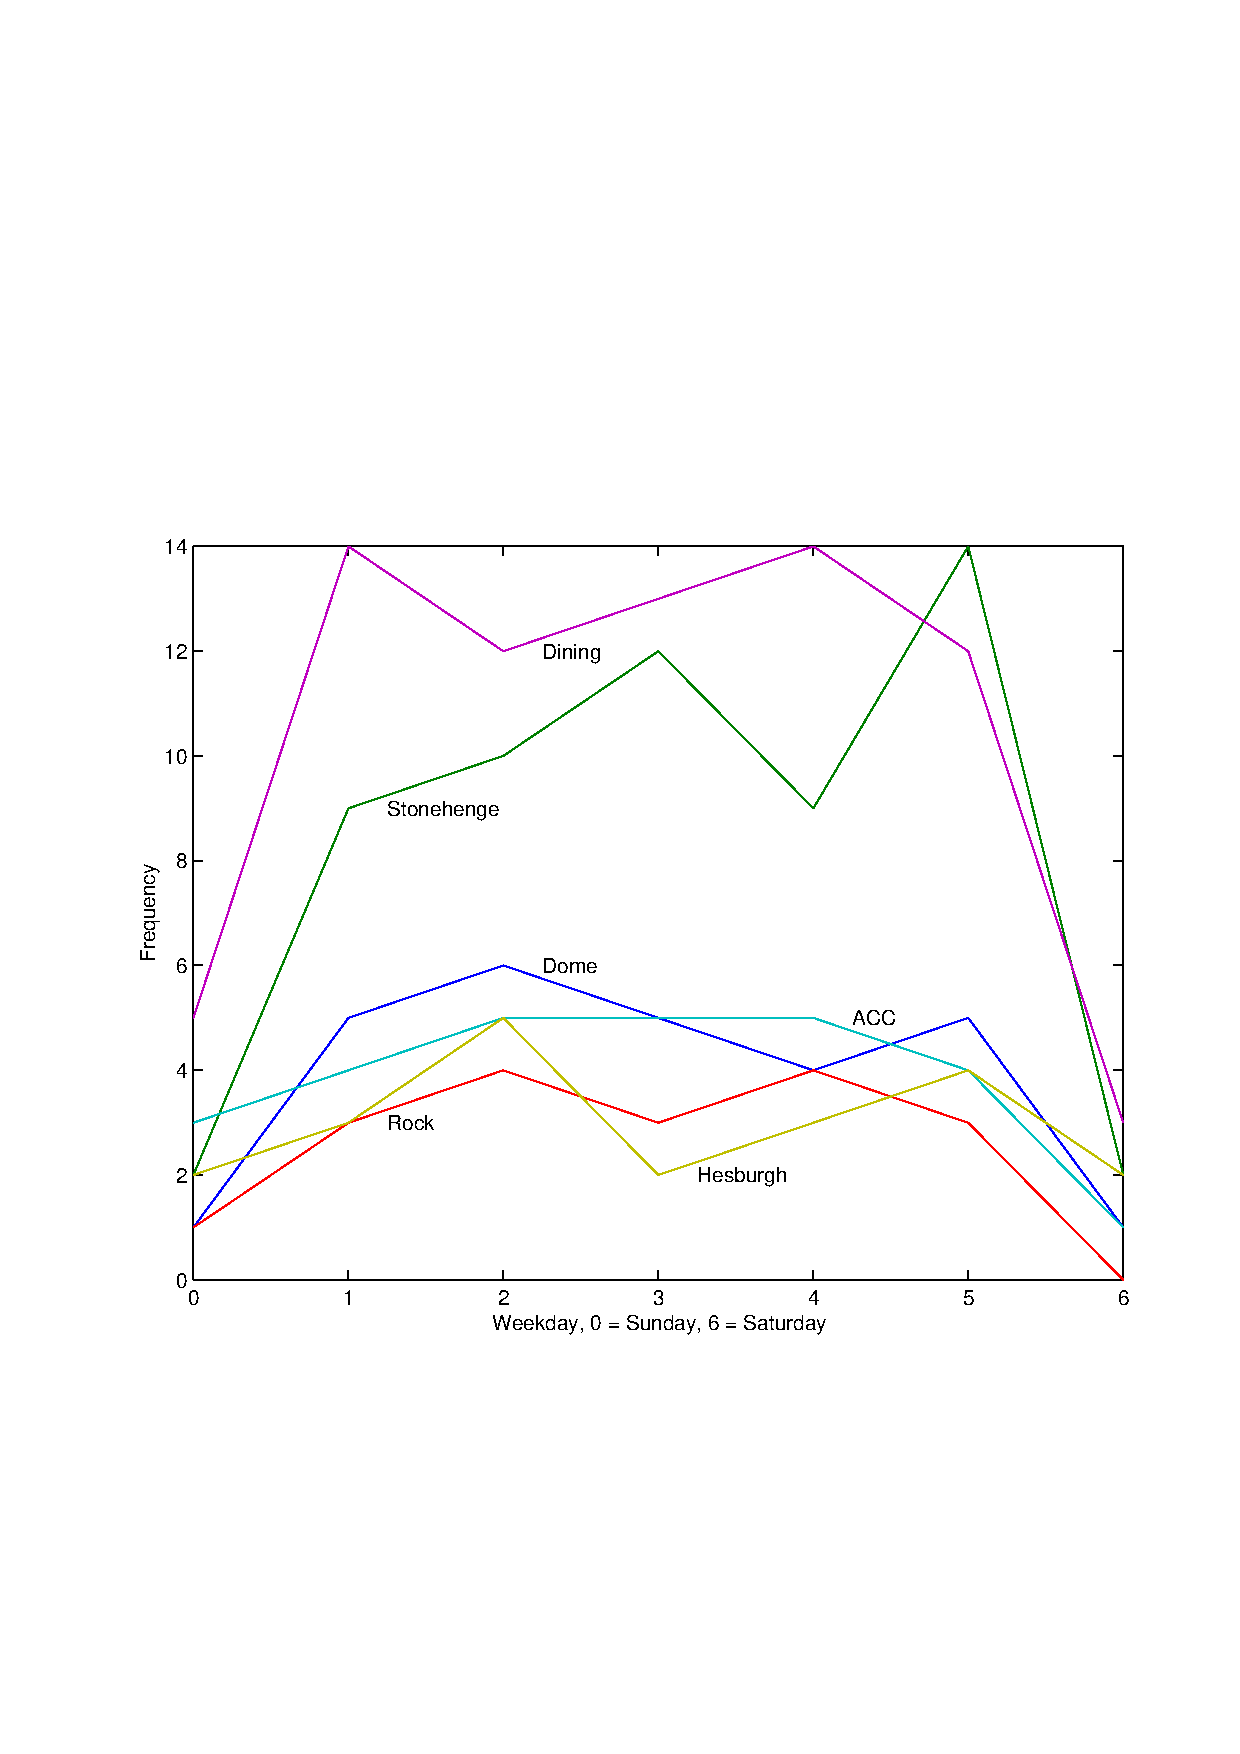
\includegraphics[scale=0.8]{sample_nd}}
    \caption{Location distributions by day of where, where the X axis
      is the weekday (0 through 6), and the Y axis is the sighting
      frequency}
    \label{fig:bogus3}
  \end{center}
\end{figure}

Gnus typically tend to come out when there are large gatherings of
humans with food.  Gnus work very hard at providing us with all the
things that we like (trees, dirt, air, etc.), and so we should freely
give them food.  They will come up and stand a respectful distance
away from you, waiting to see if they will be rewarded for their
efforts.  If you offer some food, they will take it and back off a
respectful distance in order to consume their food while leaving you
to your ``personal space.''  

\section{Groovin' Gnus}
\label{sec:groovin-gnus}

Gnus do tend to stay away from humans in their normal day-to-day
workings.  This is mainly because humans don't, for the most part,
understand what they are doing.  If a Gnu is working, and a human
approaches it, the Gnu will tend to drop whatever it is doing and run
away.  This is probably do to the tendency for humans to have ``group
meetings'' and ``productivity seminars.''  Most Gnus are deathly
afraid of such overmanagement, and run at the slightest hint of it,
for fear that it will cripple their real work.

It is interesting, however, that Gnus have chosen an Institution of
Higher Education for their BOO.\footnote{Base of Operations.}  It is
often said that:
\begin{quote}
  Academic politics are the dirtiest, meanest, ugliest, and generally
  the most low-down, in-your-face, and kick-em-while-they're-down than
  anywhere else (even Washington D.C.)  because the stakes are so low.
\end{quote}
It has been hypothesized that the Gnus are subtly trying to affect a
change for the better (i.e., eliminating the overmanagement problems)
by working the very system that they are trying to change, from
within.  That is, the graduates from Notre Dame can learn from the
examples of the Gnus here, and run screaming (or chattering) at the
slightest hint of overmanagement, and let the real work proceed
unhindered.

% % uncomment the following lines,
% if using chapter-wise bibliography
%
% \bibliographystyle{ndnatbib}
% \bibliography{example}

% \chapter{فضاهای فشرده پایدار و فضاهای مرتب فشرده}
\thispagestyle{empty}
\section{فضاهای فشرده پایدار}
یک فضای توپولوژیک جزئاً مرتب (یا به طور خلاصه، فضای مرتب)، از دیدگاه آبرامسکی
\cite{abramsky2}،
مجموعه‌ای مانند $ X $ همراه 
با یک توپولوژی $ \mathcal{O} $ و یک ترتیب $ \leq $ است به طوری که گراف ترتیب در $X\times X  $ بسته باشد. بنابراین ...
\section{فضاهای مرتب فشرده}
در این  بخش به بیان ...
% \chapter{اندازه‌ها و ارزیابی‌ها}
\thispagestyle{empty}
\section{اندازه‌ها و تابعی‌های خطی مثبت روی $\mathrm{C(X)}$}
فرض کنید $X$ یک فضای توپولوژیکی روی ...
\section{تابعی‌های خطی}
در این بخش ...
% \bibliographystyle{plain}
% \bibliography{xbib}
% \end{document}
% \end{verbatim}
% \hrulefill
% \caption{Example for using \package{srcltx.sty} with the WinEdt error tracking features.}\label{ex}
% \end{figure}
% 
% \subsection{Commands}
% \begin{descr}
% 
% \item[\Com{Input}\marg{filename}] In order to keep track
% 	   of the current filename, the \LaTeX\ commands
% 	   \Com{include}\marg{filename} and \Com{input}\marg{filename}
% 	   are overloaded (note the braces enclosing the filename argument).  The
% 	   \Com{input} command where the filename can be specified
% 	   without any delimiters is a \TeX\ primitive command that can
% 	   not be overloaded easily.  Therefore the package provides an
% 	   alternative command |\Input| which you should use in Plain
% 	   \TeX\ instead of \Com{input} if you want the specials in such
% 	   files to point to the correct filename.  For \LaTeX, you
% 	   should always use the version with braces:
% 	   \Com{input}\marg{filename}.  \emph{Note}: For Winedt, you will
% 	   also need to specify the file name extension (e.g.
% 	   \file{.tex}) in the argument of this command.
% 
% \item[\Com{MainFile}] Usually the \TeX\ primitive |\jobname| contains the name of the
% 	   ``main'' TeX file, without the filename extension `\file{.tex}'.
% 	   Accordingly, |\MainFile| is defined as |\jobname.tex|. 
% 	   If you have a very awkward \TeX\ implementation that already adds the extension
% 	   to |\jobname|, you compensate for this by redefining this command as follows
%          (after loading \package{srcltx.sty}):
% 
% 	   \noindent\begin{tabular}{@{}l@{}}
% 	   |\def\MainFile{\jobname}|
% 	   \end{tabular}
%
% \item[\Com{srcIncludeHook}] This is a hook that is called by the \Com{include}
%          command. It takes the argument of that command and sets \Com{CurrentInput}
%	   to that argument (or a modified version thereof); the content of \Com{CurrentInput}
%	   is used as file name in the source specials. This hook can be used
%          to write a customized file name into the source specials. For example,
%          if the \file{.tex} source file is automatically generated from some
%          master document, the source specials in the DVI file could point
%          to that master document instead of the generated \file{.tex} file.
%
%          Its default definition is:
%
% 	   \noindent\begin{tabular}{@{}l@{}}
%               |\newcommand*\srcIncludeHook[1]{% |\\
%               |    \protected@xdef\CurrentInput{#1.tex}}|
% 	   \end{tabular}
%
%	   \noindent
%	   (for \LaTeX, similar with \Com{def} for \TeX).
%
% \item[\Com{srcInputHook}] This is similar to \Com{srcIncludeHook}, but for the \Com{input}
%	   command.
%
%          Its default definition is:
%
% 	   \noindent\begin{tabular}{@{}l@{}}
%               |\newcommand*\srcInputHook[1]{\src@getfilename@with@ext{#1}}|
% 	   \end{tabular}
%
%	   \noindent
%	   (for \LaTeX, similar with \Com{def} for \TeX); \Com{src@getfilename@with@ext}
%	   will append a `.tex' extension to the filename if it doesn't already end
%	   with `.tex'.
%
% \item[\Com{SRCOKtrue}, \Com{SRCOKfalse}] You can use these commands to
% 	   activate\slash deactivate source specials at any place in your
% 	   document, e.g. when you experience problems with some special
% 	   constructions (see also `Bugs and Restrictions' in section
% 	   \ref{sec:bugs}).
% 	   
% \end{descr}
% 
% \section{Bugs and Restrictions}\label{sec:bugs}
% 
% Since this macro package overloads some internal \LaTeX\ commands, it
% is not as robust as one might wish, and might interact badly with other
% packages. Furthermore, the spacing might be altered by using the
% package; for example, with the \file{amsmath} documentation \file{amsldoc.tex},
% the bibliography is shifted from the bottom of page 31 to page 32.
% Therefore you should comment out the package or disable it with the
% \texttt{inactive} option when preparing the final version of your document.
% 
% A somewhat more robust method of inserting source specials is to use \TeX\
% (the program) instead of a macro solution. Some \TeX\ implementations
% provide a command line option for this.\footnote{%
% E.g. a `\file{-src}' option is available in Mik\TeX\ from version 1.20 upwards,
% or in te\TeX\ from version beta-20011103 or teTeX-2.0 upwards. See the manual of your
% \TeX\ implementation for details on this.}
% You can still load \package{srcltx.sty} with the `\texttt{inactive}' option to enable
% the WinEdt error tracking features when needed.
% 
% This section lists known incompatibilities with other packages and workarounds for these.
% If you know of any other problems, please send a bug report to
% \href{mailto:stefanulrich@users.sourceforge.net}{\texttt{<stefanulrich@users.sourceforge.net>}}.
% \begin{description}
% \item[{\normalfont\package{soul.sty}:}] Active source specials inside
% 	  the soul tokenization routine may lead to a `reconstruction failed'
% 	  error. As a workaround, the internal command |\SOUL@| is overloaded
% 	  by \package{srcltx}. With the Plain \TeX\ version, \package{srctex.sty}
% 	  needs to be loaded \emph{after} \package{soul.sty} to make this work.
% \item[{\normalfont\package{syntax.sty}:}] This style does extensive parsing
% 	  of the input inside its `grammar' environment, which is incompatible
% 	  with \package{srcltx.sty}.
% \end{description}
% 
% \section{Related Packages}
% 
% Heiko Oberdiek's \package{vpe.sty} provides source specials for
% forward search in PDF files. To our knowledge there exists no
% implementation for reverse search with PDF viewers, or inverse search
% in Postscript documents.
% 
% \section{History}
% 
% This package was originally written by A.~Simonic, the author of the WinEdt Shell,
% to implement source file tracking and DVI source specials
% for \TeX. D.~P.~Carlisle and B.~K.~Horn have contributed bug
% fixes. Further changes and conversion to \file{ltxdoc} format by S.~Ulrich.
% Thanks for patches and suggestions to: A.~Cherepanov, J.~Rawnsley, D.~Kastrup,
% D.~Arseneau, M.~S.~Gr\o nsleth and R.~Hemmecke.
% 
%
% \StopEventually{}
% \section{Implementation}
%
% \changes{v1.6}{2006/11/12}{Provide \Com{srcInputHook} and \Com{srcIncludeHook} for changing
%		the input filename on-the-fly,
%               as requested by Ralf Hemmecke for his Axiom and ALLPROSE packages.
%               Also fixed \Com{src@getfilename@with@ext} so that it doesn't append `.tex' any
%               more in cases where the filename had a complex extension (e.g. `foo.bar.tex')
%               with the last element `.tex'.}
% \changes{v1.5}{2004/10/05}{Fixed version number in documentation, and made \Com{input} append .tex
%		extension if not yet present (feature requested by Martin Sigurd Gr\o nsleth).}
% \changes{v1.4}{2004/05/15}{Fixed \Com{everypar} hook, as suggested by David Kastrup in comp.text.tex,
%		for compatibility with chapterbib.sty}
% \changes{v1.3}{2003/03/10}{Also hook into \Com{everydisplay}; unreleased since this change broke
%		regression for gentle.tex}
% \changes{v1.2c}{2002/03/01}{Added the `nowinedt' option}
% \changes{v1.2b}{2002/01/23}{Fixed spurious space introduced by uncommented linebreak}
% \changes{v1.2}{2002/01/21}{Replace stack by macro solution, as suggested by
%               Alexander Cherepanov (cherepan at mccme.ru).
%               Also overload LaTeX's \Com{input} command.}
% \changes{v1.1a}{2001/07/14}{Minor fixes in the documentation.}
% \changes{v1.1}{2001/03/31}{SU: converted to ltxdoc format, changed the
%                            push\slash pop commands to use a `real' stack,
%                            other minor modifications}
% \changes{v1.002}{1999/09/03}{modified to change \Com{everypar}, by David Carlisle}
% \changes{v1.001}{1998/12/23}{modified to change \Com{output}, by Berthold Horn}
%
%
%    \begin{macrocode}
%<*package>
%<tex>\catcode`\@=11
\newif\ifSRCOK \SRCOKtrue
\newif\ifsrc@debug@
\newif\ifsrc@dviwin@
\newif\ifsrc@winedt@\src@winedt@true
\newif\ifsrc@everypar@\src@everypar@true
\newif\ifsrc@everymath@\src@everymath@true
%<*latex>
\RequirePackage{ifthen}
\DeclareOption{active}{\SRCOKtrue}
\DeclareOption{inactive}{\SRCOKfalse}
\DeclareOption{nowinedt}{\src@winedt@false}
\DeclareOption{debug}{\src@debug@true}
\DeclareOption{nopar}{\global\src@everypar@false}
\DeclareOption{nomath}{\global\src@everymath@false}
%</latex>
%<*tex>
\def\SRCdebug{\src@debug@true}
\def\SRCnopar{\src@everypar@false}
\def\SRCnomath{\src@everymath@false}
\def\typeout#1{{\newlinechar`\^^J\message{#1^^J}}}
\def\AtBeginDocument#1{#1}
%</tex>
%<latex>\newcommand*\src@maybe@space{}
\let\src@maybe@space\space
%<latex>\DeclareOption{dviwin}{\let\src@maybe@space\relax}
%    \end{macrocode}
%    SU: Originally the default was |\ExecuteOptions{inactive}|, but this
%    was rather unintuitive, so I changed it.
%    \begin{macrocode}
%<latex>\ExecuteOptions{active}
%<latex>\ProcessOptions
\newcount\src@lastline
\global\src@lastline=-1
%<latex>\newcommand*\src@debug{}
\def\src@debug#1{\ifsrc@debug@\typeout{DBG: |#1|}\fi}
%    \end{macrocode}
%    \begin{macro}{\MainFile}
%    This is for compatibility with \TeX\ implementations that add already
%    the `\file{.tex}' extension to \Com{jobname} (very rare):
%    \begin{macrocode}
%<latex>\newcommand*\MainFile{}
\def\MainFile{\jobname.tex}
%    \end{macrocode}
%    \end{macro}
%    \begin{macro}{\CurrentInput}
%    Used to keep track of current input file name:
%    \begin{macrocode}
%<latex>\newcommand*\CurrentInput{}
\gdef\CurrentInput{\MainFile}
%    \end{macrocode}
%    \end{macro}
%    Command to customize WinEdt's log mode, and enable its input file
%    tracking. This is switched off when the option \texttt{nowinedt} is
%    selected.
%    \begin{macrocode}
%<latex>\newcommand*\WinEdt{}
\def\WinEdt#1{\ifsrc@winedt@\typeout{:#1}\fi}
%    \end{macrocode}
%    A hook for \package{soul}, which might otherwise break with
%    a `reconstruction failed' error:
%    \begin{macrocode}
%<latex>\newcommand\src@AfterFi{}
\def\src@AfterFi#1\fi{\fi#1}
\AtBeginDocument{%
%<latex>    \@ifpackageloaded{soul}{%
%<tex>\ifx\SOUL@\relax
%<tex>\else
        \let\src@SOUL@\SOUL@
        \def\SOUL@#1{%
            \ifSRCOK
                \SRCOKfalse\src@SOUL@{#1}\SRCOKtrue
            \else
                \src@AfterFi\src@SOUL@{#1}%
            \fi
        }%
%<tex>\fi
%<latex>    }{}%
}
%    \end{macrocode}
%    \begin{macro}{\srcIncludeHook}
%    Hook to set the name of the current input file (\Com{CurrentInput}) for the \Com{include} command.
%    \begin{macrocode}
%<latex>\newcommand*\srcIncludeHook[1]{\protected@xdef\CurrentInput{#1.tex}}
%<tex>\def\srcIncludeHook#1{\xdef\CurrentInput{#1.tex}}
%    \end{macrocode}
%    \end{macro}
%
%    \begin{macro}{\srcInputHook}
%    Hook to set the name of the current input file (\Com{CurrentInput}) for the \Com{Input} command.
%    \begin{macrocode}
%<latex>\newcommand*\srcInputHook[1]{%
%<tex>\def\srcInputHook#1{%
    \src@getfilename@with@ext{#1}%
}
%    \end{macrocode}
%    \end{macro}
%
%    \begin{macro}{\src@spec}
%    Macro that actually inserts the special.
%    \begin{macrocode}
%<latex>\newcommand*\src@spec{}
\def\src@spec{%
    \ifSRCOK
        \ifnum\inputlineno>\src@lastline
            \global\src@lastline=\inputlineno
            \src@debug{%
                src:\the\inputlineno\src@maybe@space\CurrentInput}%
            \special{src:\the\inputlineno\src@maybe@space\CurrentInput}%
        \fi
    \fi
}
%    \end{macrocode}
%    \end{macro}
%
%    \begin{macro}{\src@before@file@hook}
%    \begin{macro}{\src@after@file@hook}
%    Hooks executed before and after a level of input happens:
%    \begin{macrocode}
%<latex>\newcommand\src@before@file@hook{}
%<latex>\newcommand\src@after@file@hook{}
\def\src@before@file@hook{%
    \WinEdt{<+ \CurrentInput}%
    \global\src@lastline=0
    \ifSRCOK\special{src:1\src@maybe@space\CurrentInput}\fi
}
\def\src@after@file@hook#1{%
    \WinEdt{<-}%
    \global\src@lastline=\inputlineno
    \global\advance\src@lastline by -1%
    \gdef\CurrentInput{#1}%
    \src@spec
}
%    \end{macrocode}
%    \end{macro}
%    \end{macro}
%
%    \begin{macro}{\src@getfilename@with@ext}
%    Check if \verb+#1+ has the extension `.tex', and if not, append it, saving the
%    result to \Com{CurrentInput}. \emph{Warning:} This does not completely mimick
%    the behaviour of \Com{input}, since it also expands a filename `foo.sty' to
%    `foo.sty.tex' even if `foo.sty' exists. However in the context of this
%    package that doesn't matter much since we assume that files that don't have
%    a `.tex' extension won't create any content in the DVI file.
%
%    The command \Com{src@extensions@path} is similar to \Com{filename@parse}
%    from \file{latex.ltx}.
%    \begin{macrocode}
%<*latex>
\newcommand*\src@fname{}%
\newcommand*\src@tempa{}%
\newcommand*\src@extensions@path{}%
\newcommand*\src@getfilename@with@ext{}%
%</latex>
%<*tex>
\def\src@tempa{}%
%</tex>
\def\src@extensions@path#1.#2\end{%
%<*latex>
   \ifthenelse{\equal{#2}{}}{%
       \protected@edef\src@extensions@last{#1}%
       \let\src@tempa\relax
   }{%
       \def\src@tempa{\src@extensions@path#2\end}%
   }%
%</latex>
%<*tex>
   \ifx\\#2\\
       \edef\src@extensions@last{#1}%
       \let\src@tempa\relax
   \else
       \def\src@tempa{\src@extensions@path#2\end}%
   \fi
%</tex>
   \src@tempa
}
\def\src@getfilename@with@ext#1{%
    \expandafter\src@extensions@path#1.\end
%<*latex>
    \ifthenelse{\equal{\src@extensions@last}{tex}}{%
        \protected@xdef\CurrentInput{#1}%
    }{%
        \protected@xdef\CurrentInput{#1.tex}%
    }%
    \PackageInfo{srcltx}{Expanded filename `#1' to `\CurrentInput'}%
%</latex>
%<*tex>
    \def\src@tempa{tex}%
    \ifx\src@extensions@last\src@tempa
        \xdef\CurrentInput{#1}%
    \else
        \xdef\CurrentInput{#1.tex}%
    \fi
%</tex>
}
%    \end{macrocode}
%    \end{macro}
%
%    \begin{macro}{\include}
%    Redefine the original \Com{include} command. This is done for LaTeX only.
%    The \file{.tex} extension is added to the argument.
%    \begin{macrocode}
%<*latex>
\newcommand*\src@include{}
\newcommand*\src@@include{}
\let\src@include\include
\def\include#1{%
    \src@spec
    \clearpage
    \expandafter\src@@include\expandafter{\CurrentInput}{#1}%
}%
\def\src@@include#1#2{%
    \srcIncludeHook{#2}%
    \src@before@file@hook
    \src@include{#2}%
    \src@after@file@hook{#1}%
}
%</latex>
%    \end{macrocode}
%    \end{macro}
%
%    \begin{macro}{\input}
%    For \Com{input}, we can only overload the LaTeX syntax, i.e. the usage
%    with the argument in braces. For plain \TeX, we provide an alternative command
%    \Com{Input} that can be used instead of \Com{input}. We can't redefine
%    \Com{input}, since that is a \TeX\ primitive with a different way of parsing
%    the argument line.
%
%    A \file{.tex} extension is added to the argument if it's not already present.
%    \begin{macrocode}
%<*latex>
\newcommand*\src@input{}
\newcommand*\src@@input{}
\newcommand*\src@@@input{}
%</latex>
\let\src@input\input
%<*latex>
\def\input{\src@spec\@ifnextchar\bgroup\src@@input\@@input}%
%    \end{macrocode}
%    \Com{@@input} is \LaTeX's alias for \TeX's \Com{input} command.
%    \begin{macrocode}
\def\src@@input#1{%
    \expandafter\src@@@input\expandafter{\CurrentInput}{#1}%
}
\def\src@@@input#1#2{%
    \srcInputHook{#2}%
    \src@before@file@hook
    \src@input{#2}%
    \src@after@file@hook{#1}%
}
%</latex>
%    \end{macrocode}
%    \end{macro}
%    \begin{macro}{\Input}
%    \begin{macrocode}
%<*tex>
\def\Input#1{%
    \expandafter\src@Input\expandafter{\CurrentInput}{#1}%
}
\def\src@Input#1#2{%
    \srcInputHook{#2}%
    \src@before@file@hook
    \src@input #2
    \src@after@file@hook{#1}%
}
%</tex>
%    \end{macrocode}
%    For \LaTeX, \Com{Input} is just an alias for \Com{input}:
%    \begin{macrocode}
%<*latex>
\newcommand\Input{}
\let\Input\input
%</latex>
%    \end{macrocode}
%    \end{macro}
%    Hook into `everypar'. This should concatenate the \Com{src@spec} with
%    whatever those token lists contained before, just in case they were not
%    empty token lists (hoping that later hooks will do the same). David Kastrup
%    writes in \url{<x5ekpmxh2j.fsf@lola.goethe.zz>}:
%    \begin{quote}
%    You need \emph{two} new tokens
%    for a proper subversion.  One to save the old meaning in when the
%    package is loaded, and one to refer to [\dots] the old meaning at
%    the time the package is running, even if somebody else subverts the
%    \Com{everypar} token again.
%    \end{quote}
%    \begin{macrocode}
\ifsrc@everypar@
%<latex>    \newcommand*\src@old@everypar{}
    \let\src@old@everypar\everypar
    \newtoks\src@new@everypar
    \let\everypar\src@new@everypar
    \everypar\expandafter{\the\src@old@everypar}
    \src@old@everypar{\the\src@new@everypar\src@spec}
\fi
%    \end{macrocode}
%    Use the `nomath' option to disable the following:
%    \begin{macrocode}
\ifsrc@everymath@
%<*latex>
    \def\@tempa#1\the\everymath#2\delimiter{{#1\src@spec\the\everymath#2}}
    \frozen@everymath=\expandafter\@tempa\the\frozen@everymath\delimiter
%</latex>
%<*tex>
    \everymath\expandafter{\the\everymath\src@spec}
%</tex>
\fi
%    \end{macrocode}
%    \begin{macro}{\bibliography}
%    Hook into the \Com{bibliography} command:
%    \begin{macrocode}
%<*latex>
\newcommand*\src@bibliography{}
\newcommand*\src@@bibliography{}
\let\src@bibliography\bibliography
\def\bibliography#1{%
    \expandafter\src@@bibliography\expandafter{\CurrentInput}{#1}%
}
\def\src@@bibliography#1#2{%
%<latex>    \protected@xdef\CurrentInput{\jobname.bbl}%
%<tex>    \xdef\CurrentInput{\jobname.bbl}%
    \src@before@file@hook
    \src@bibliography{#2}%
    \src@after@file@hook{#1}%
}
%</latex>
%    \end{macrocode}
%    \end{macro}
%    Hook into output routine to turn off \Com{src@spec} while \Com{output} is active:
%    \begin{macrocode}
%<latex>\newcommand*\src@old@output{}
\let\src@old@output\output
\newtoks\src@new@output
\let\output\src@new@output
\output\expandafter{\the\src@old@output}
\src@old@output{\SRCOKfalse\the\src@new@output}
%<tex>\catcode`\@=12
%</package>
%    \end{macrocode}
% \Finale
\endinput
